\section{Výstupní data}

\subsection{Číselné výsledky}
Číselné výsledky byly formátovaně vypsány do konzole. Vzhledem k jejich rozsahu nebyly zahrnuty přímo do technické zprávy a však při každém spuštění programu si je lze snadno nechat vypsat do konzole.

\subsection{Grafické výsledky}
Grafické výsledky zahrnují vizualizace nejkratších cest v grafu a minimální kostry. Následující obrázky zobrazují jednotlivé výsledky:

\begin{figure}[H]
    \centering
    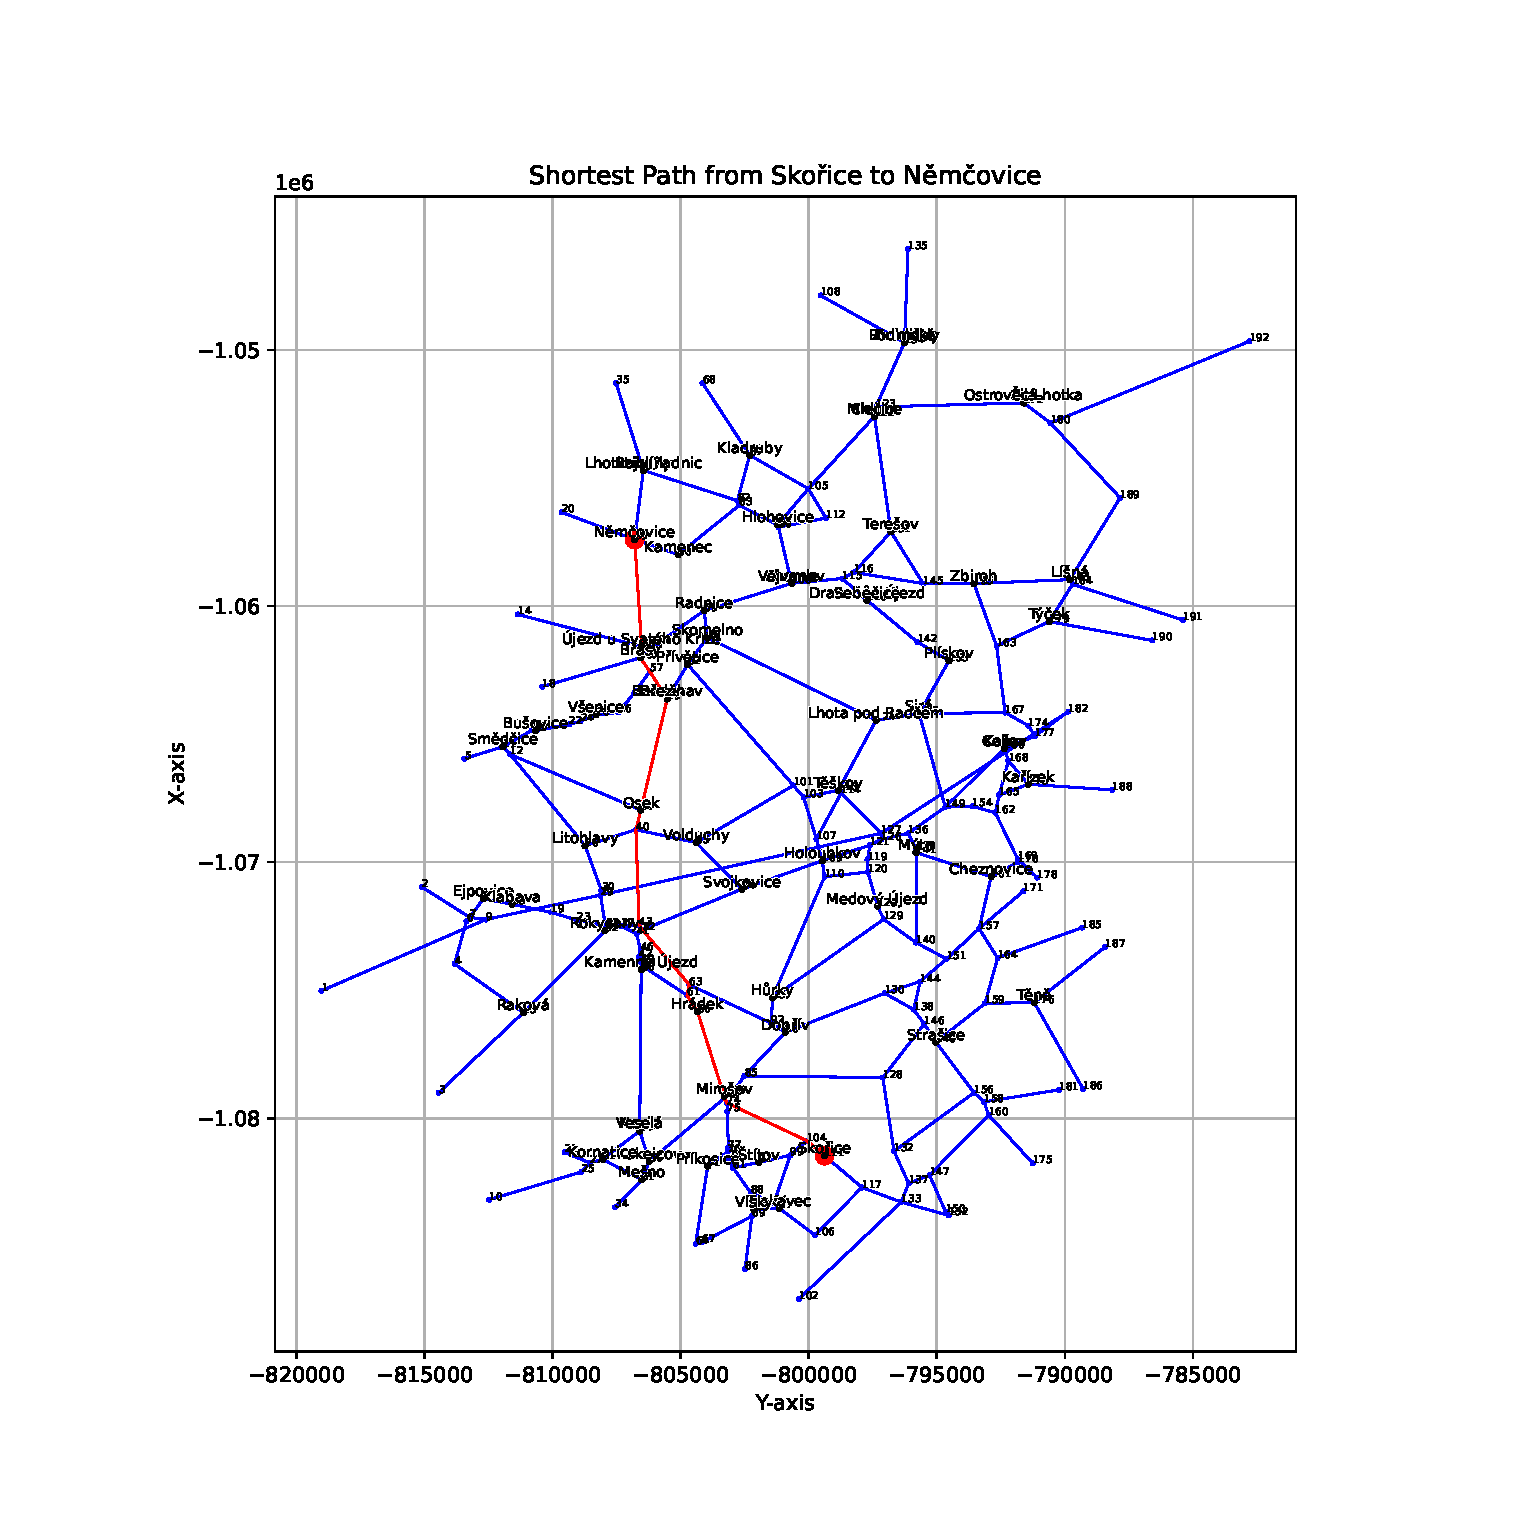
\includegraphics[width=0.65\textwidth]{images/Figure_1.eps}
    \caption{Nejkratší cesta v neohodnoceném grafu}
\end{figure}
\begin{figure}[H]
    \centering
    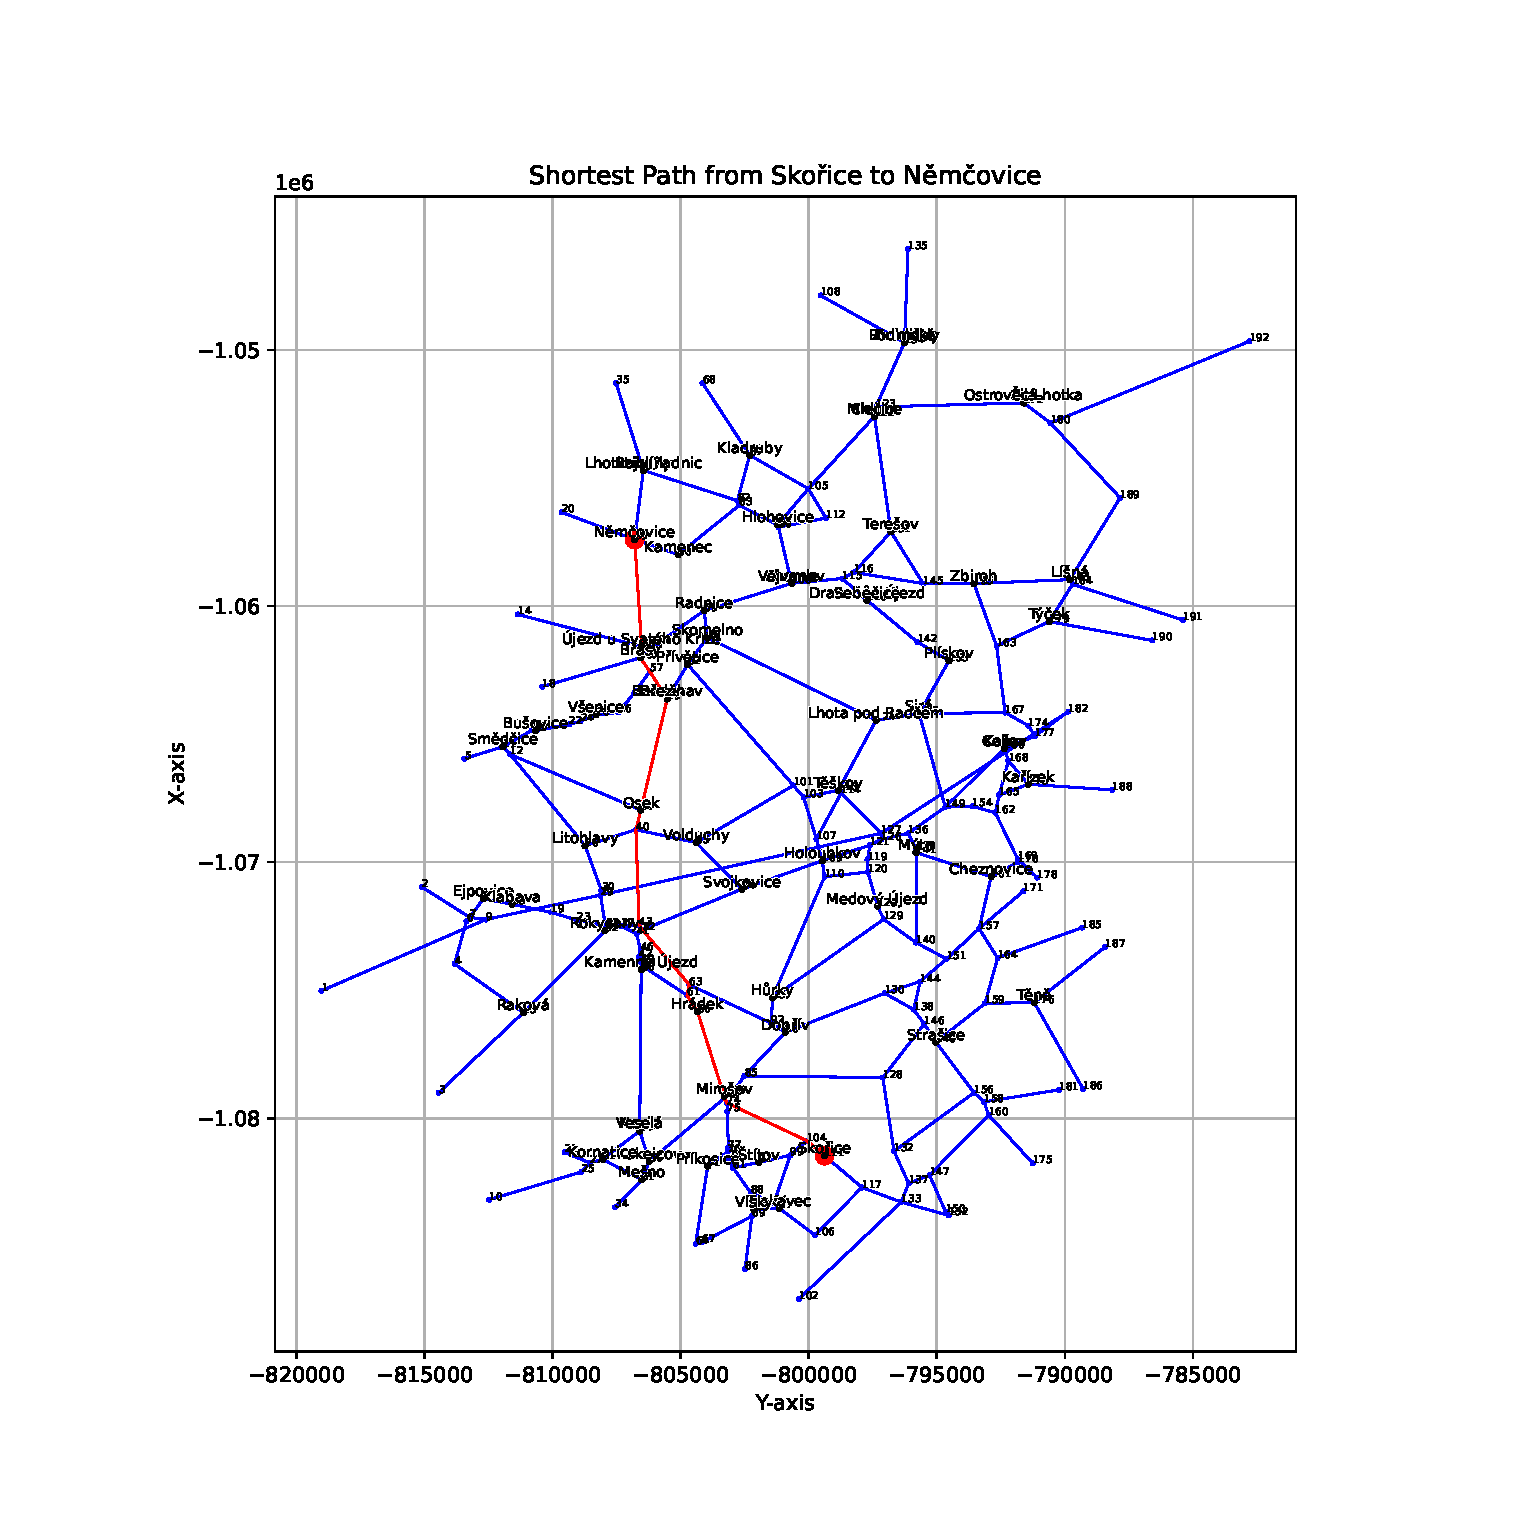
\includegraphics[width=0.65\textwidth]{images/Figure_1_curvature.eps}
    \caption{Nejkratší cesta v ohodnoceném grafu podle klikatosti}
\end{figure}
\begin{figure}[H]
    \centering
    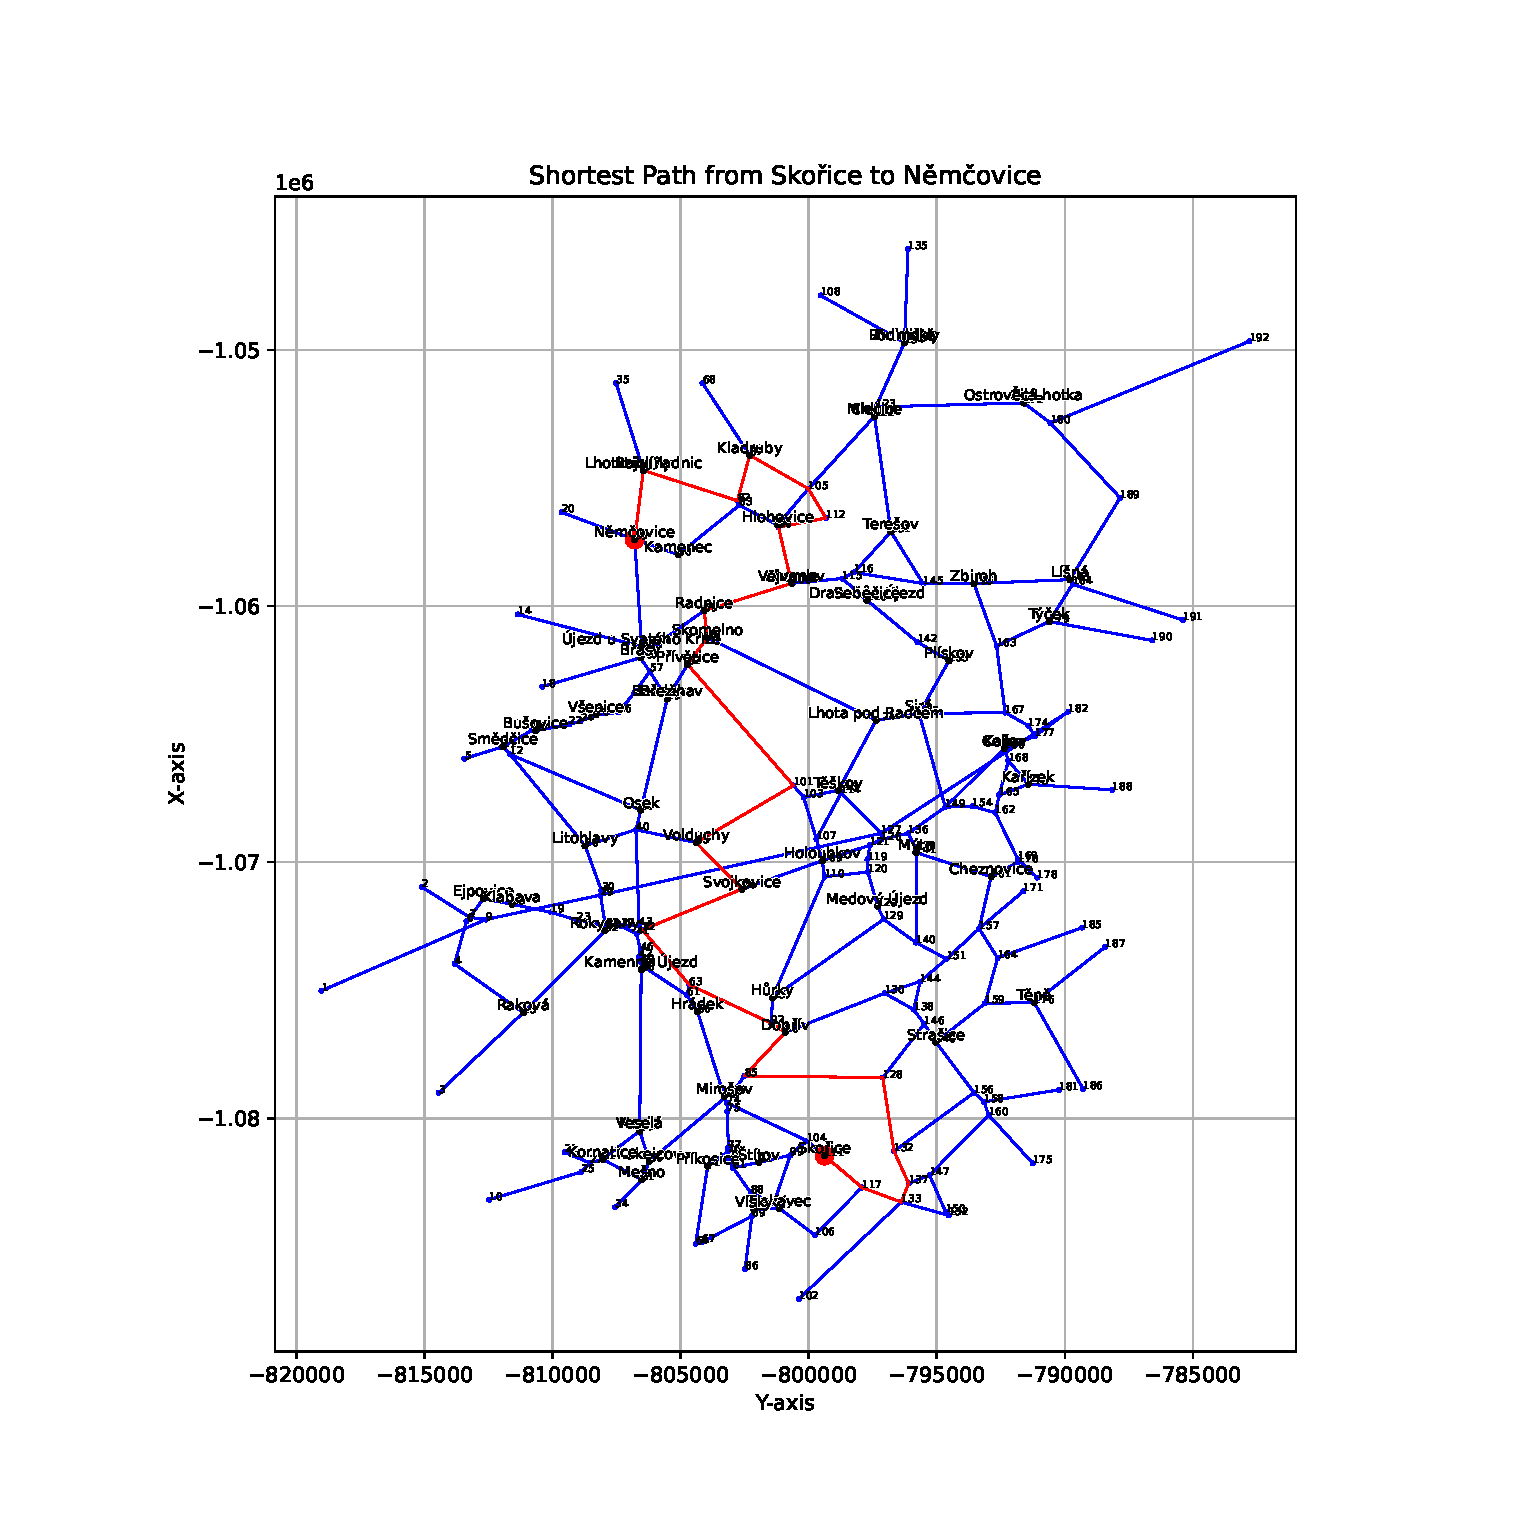
\includegraphics[width=0.65\textwidth]{images/Figure_1_length.eps}
    \caption{Nejkratší cesta v ohodnoceném grafu podle délky}
\end{figure}
\begin{figure}[H]
    \centering
    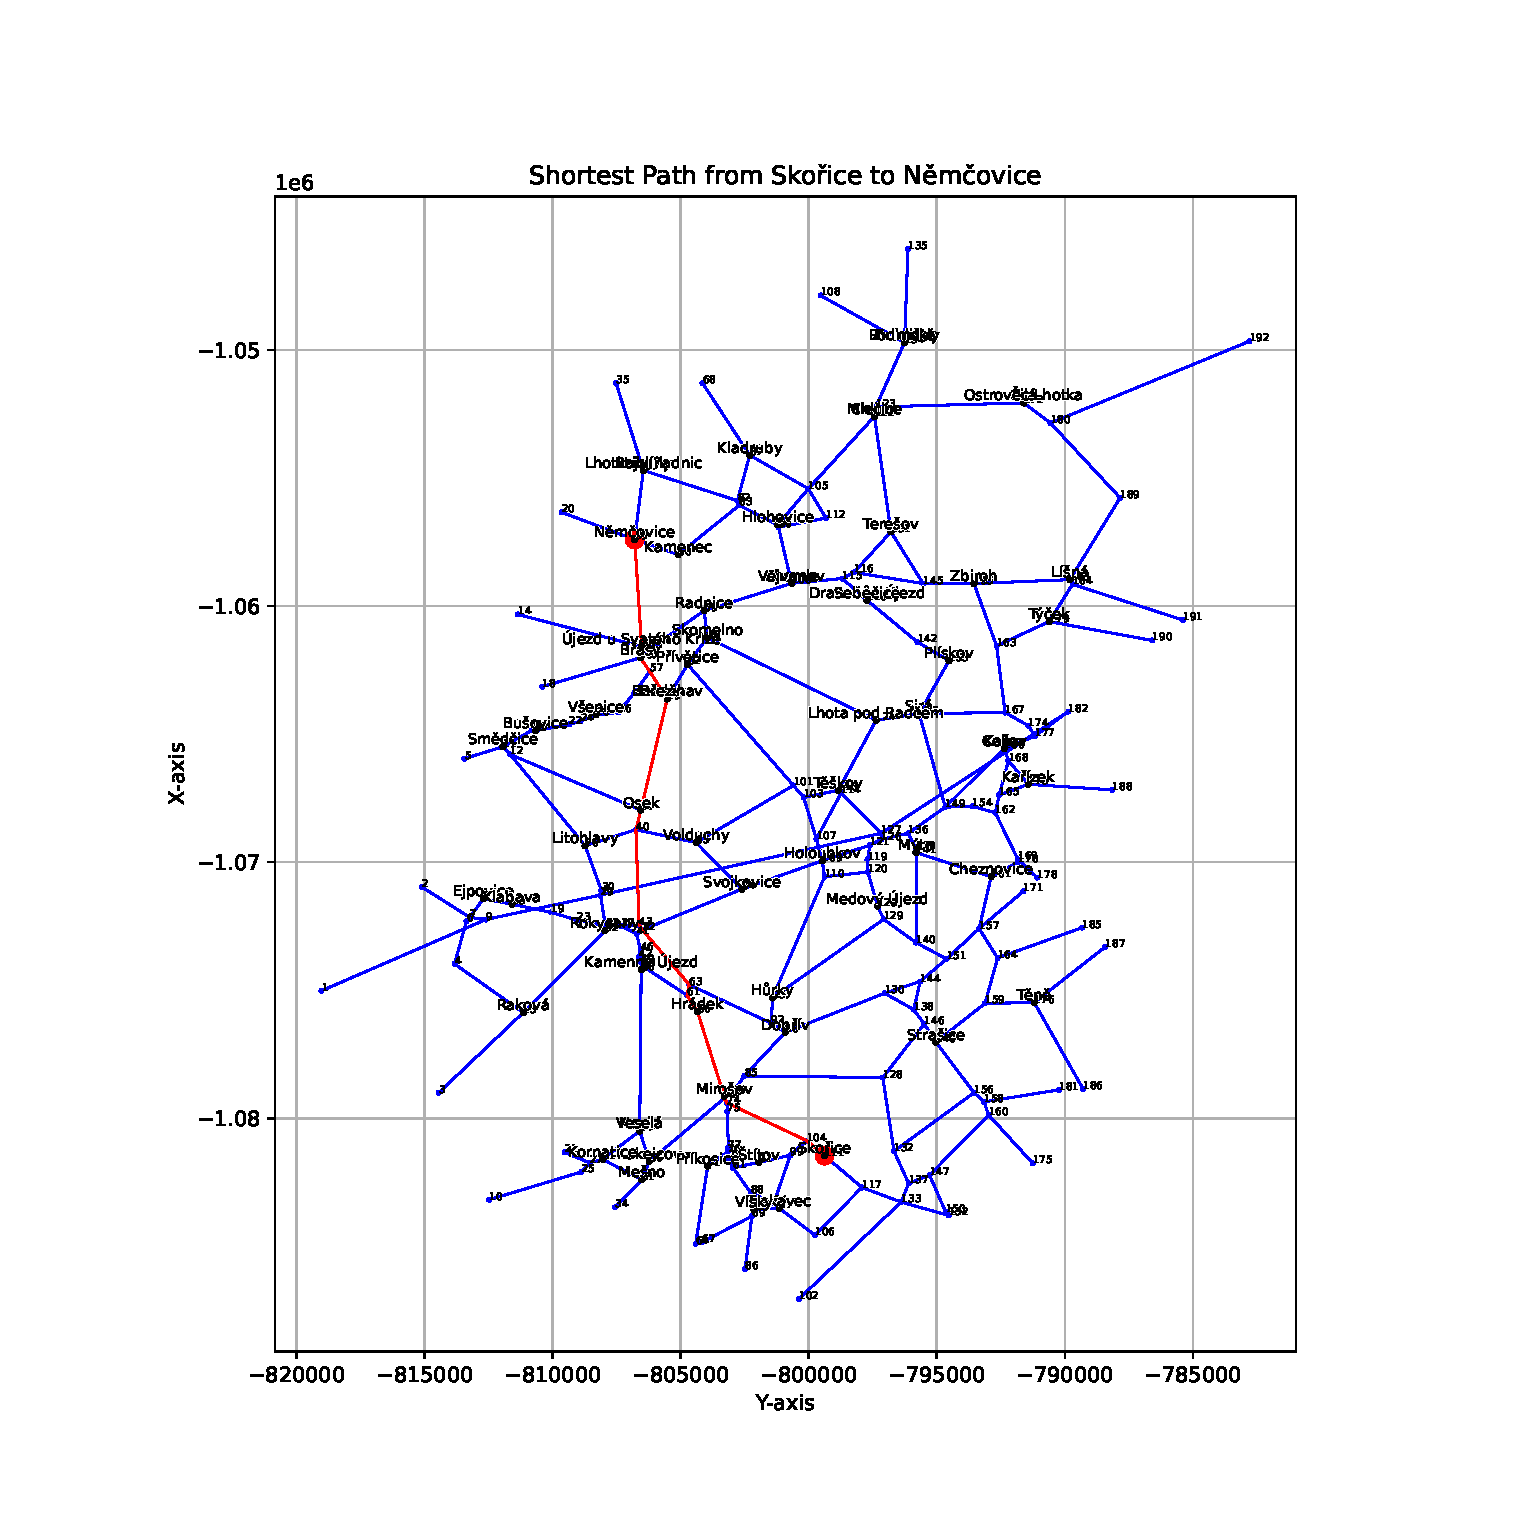
\includegraphics[width=0.65\textwidth]{images/Figure_1_speed.eps}
    \caption{Nejkratší cesta v ohodnoceném grafu podle návrhové rychlosti}
\end{figure}
%%%%%%%%%%%%%%%%%%%%%%%%%%%%%%%%%%%%%%%%%%%%%%%%%%%%%%%%%%%%%%%%%%%%%%%%%%%%%%%
\begin{figure}[H]
    \centering
    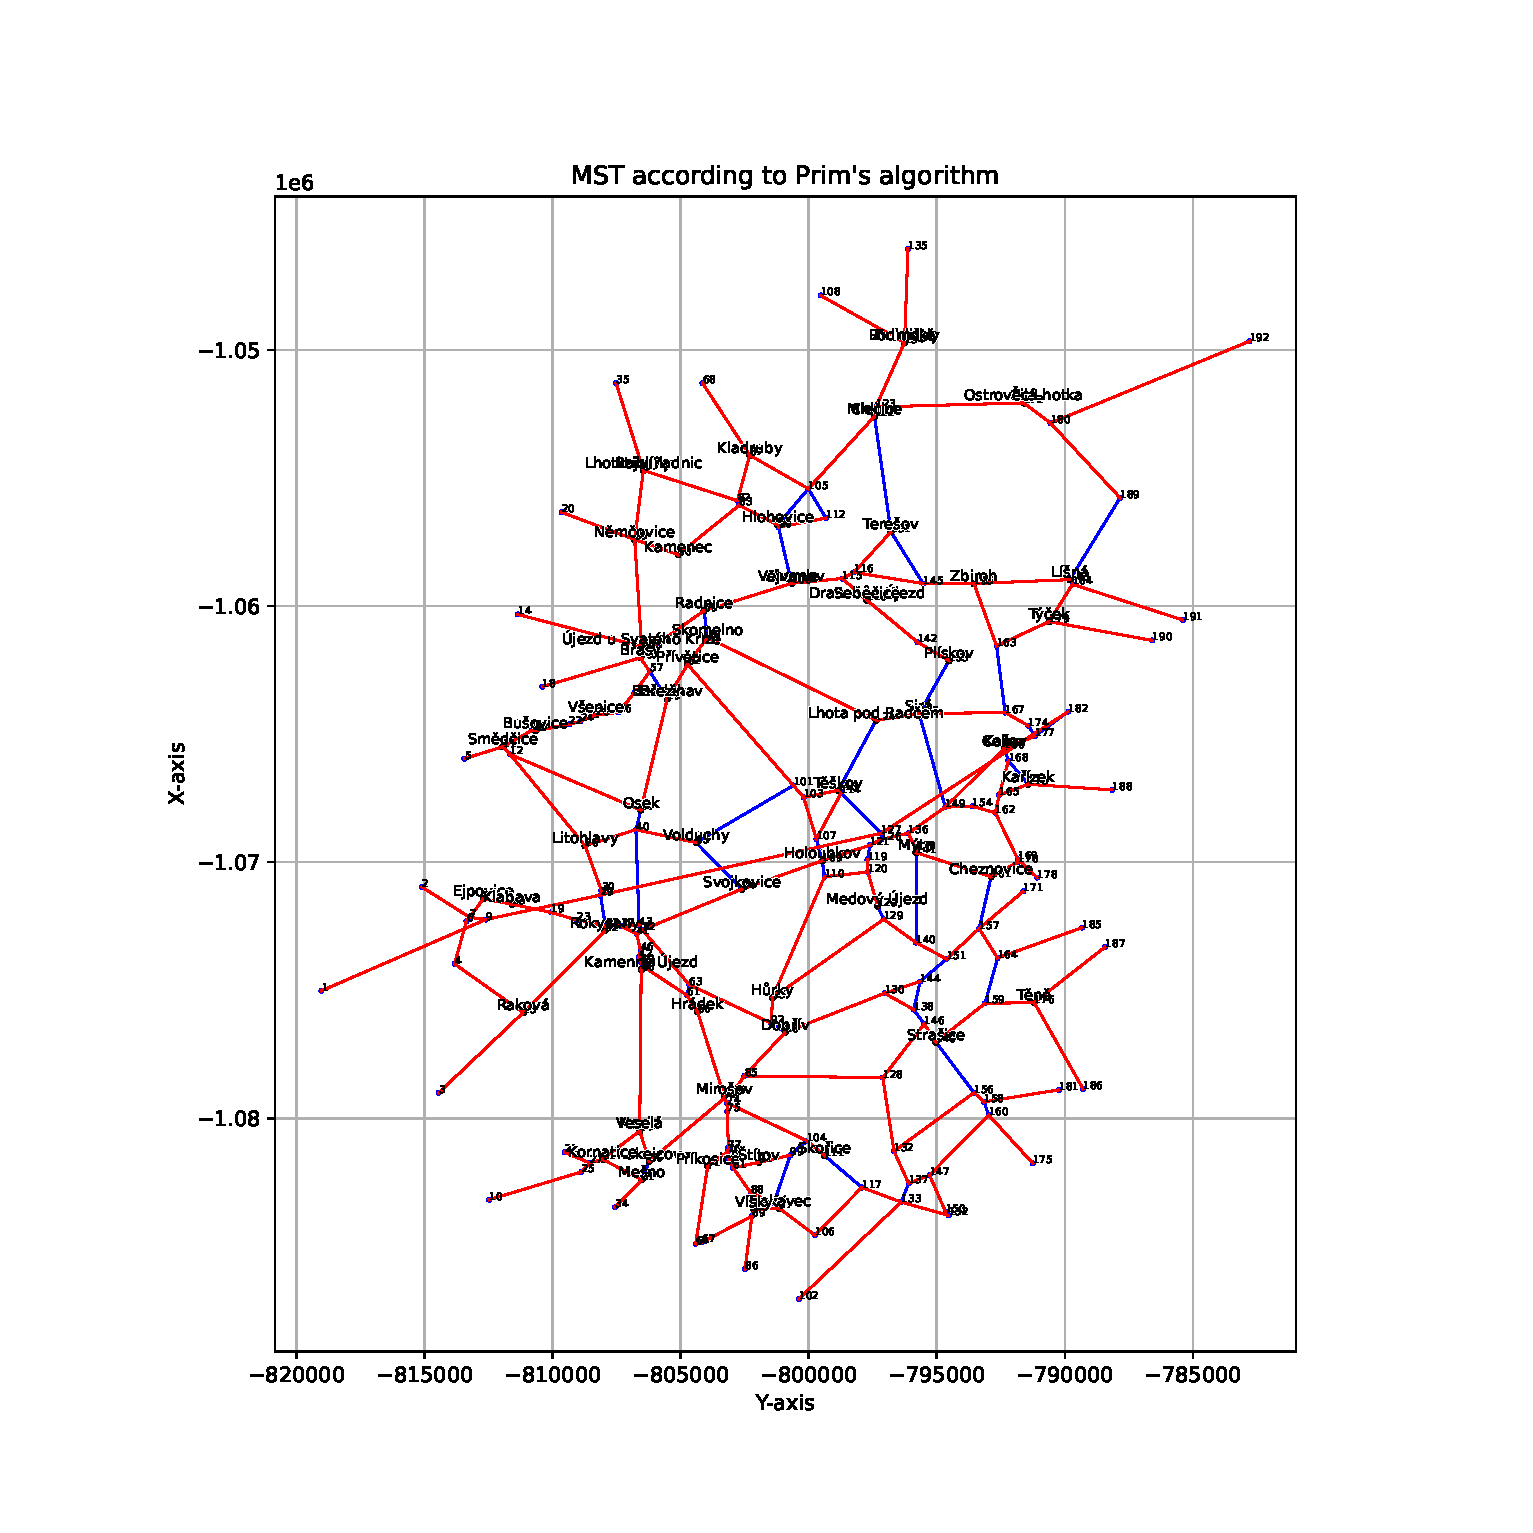
\includegraphics[width=0.65\textwidth]{images/Figure_2.eps}
    \caption{Minimální kostra neohodnoceného grafu podle Primova algoritmu}
\end{figure}


\begin{figure}[H]
    \centering
    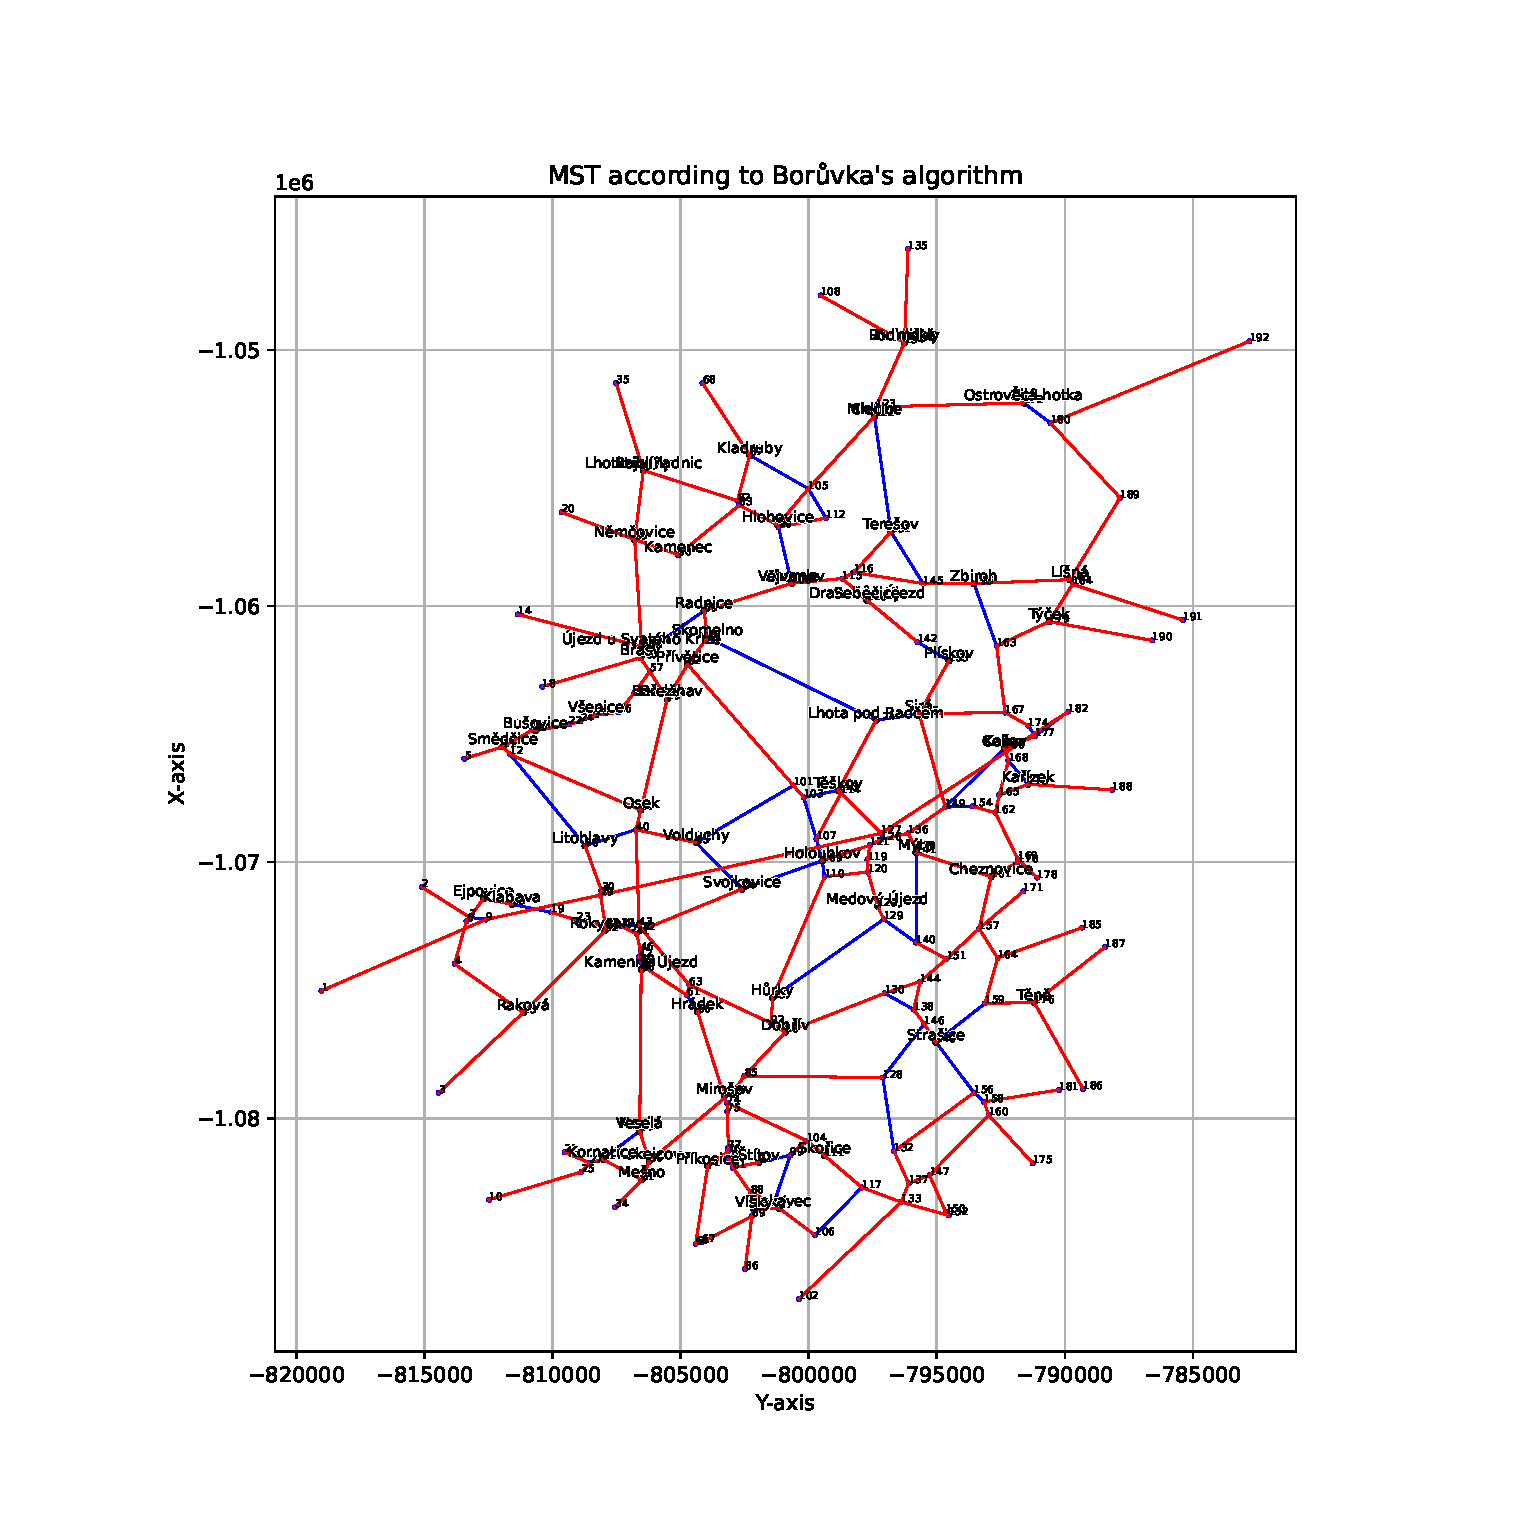
\includegraphics[width=0.65\textwidth]{images/Figure_3.eps}
    \caption{Minimální kostra neohodnoceného grafu podle Borůvkova algoritmu}
\end{figure}
%%%%%%%%%%%%%%%%%%%%%%%%%%%%%%%%%%%%%%%%%%%%%%%%%%%%%%%%%%%%%%%%%%%%%%%%%%%%%%%
\begin{figure}[H]
    \centering
    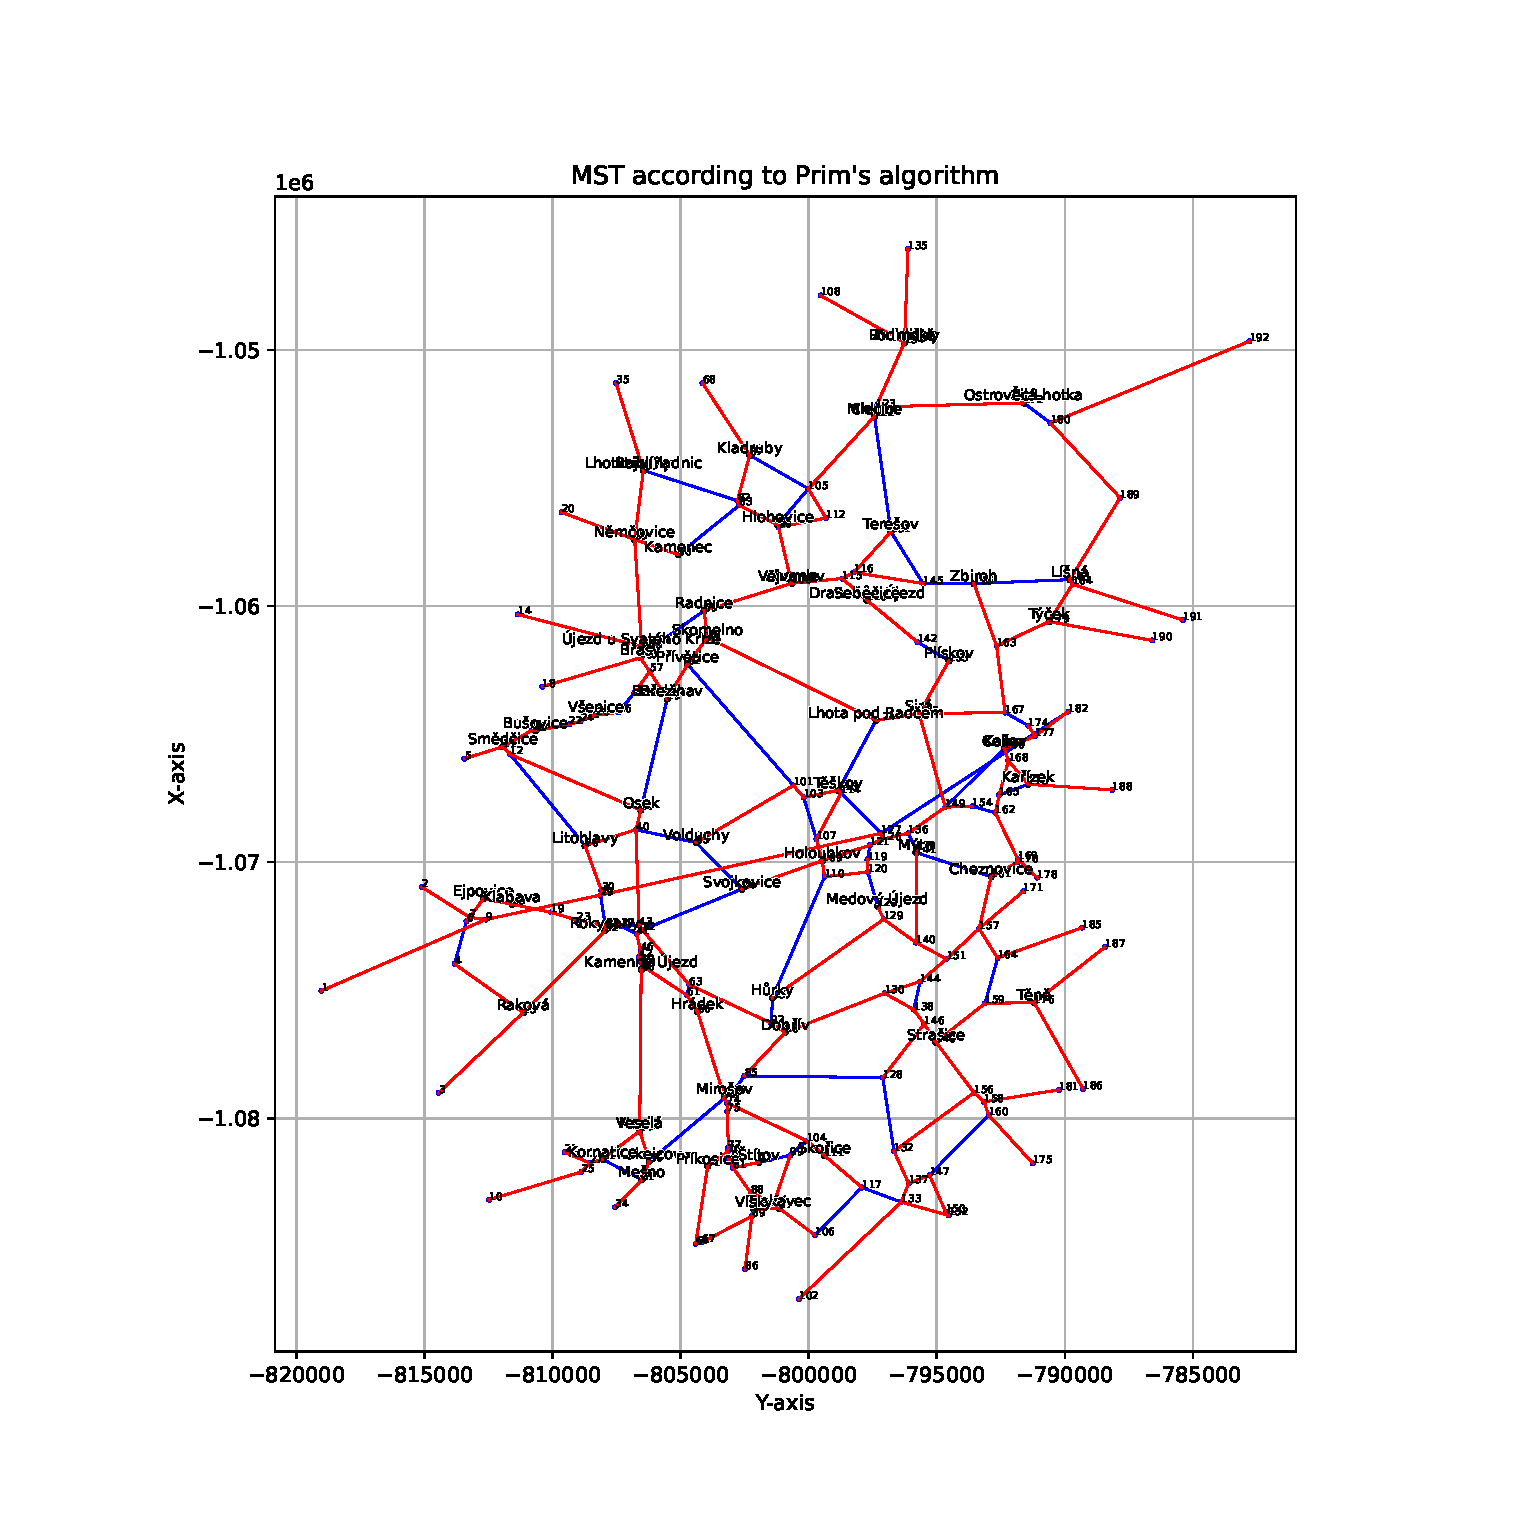
\includegraphics[width=0.65\textwidth]{images/Figure_2_curvature.eps}
    \caption{Minimální kostra v ohodnoceném grafu podle klikatosti podle Primova algoritmu}
\end{figure}
\begin{figure}[H]
    \centering
    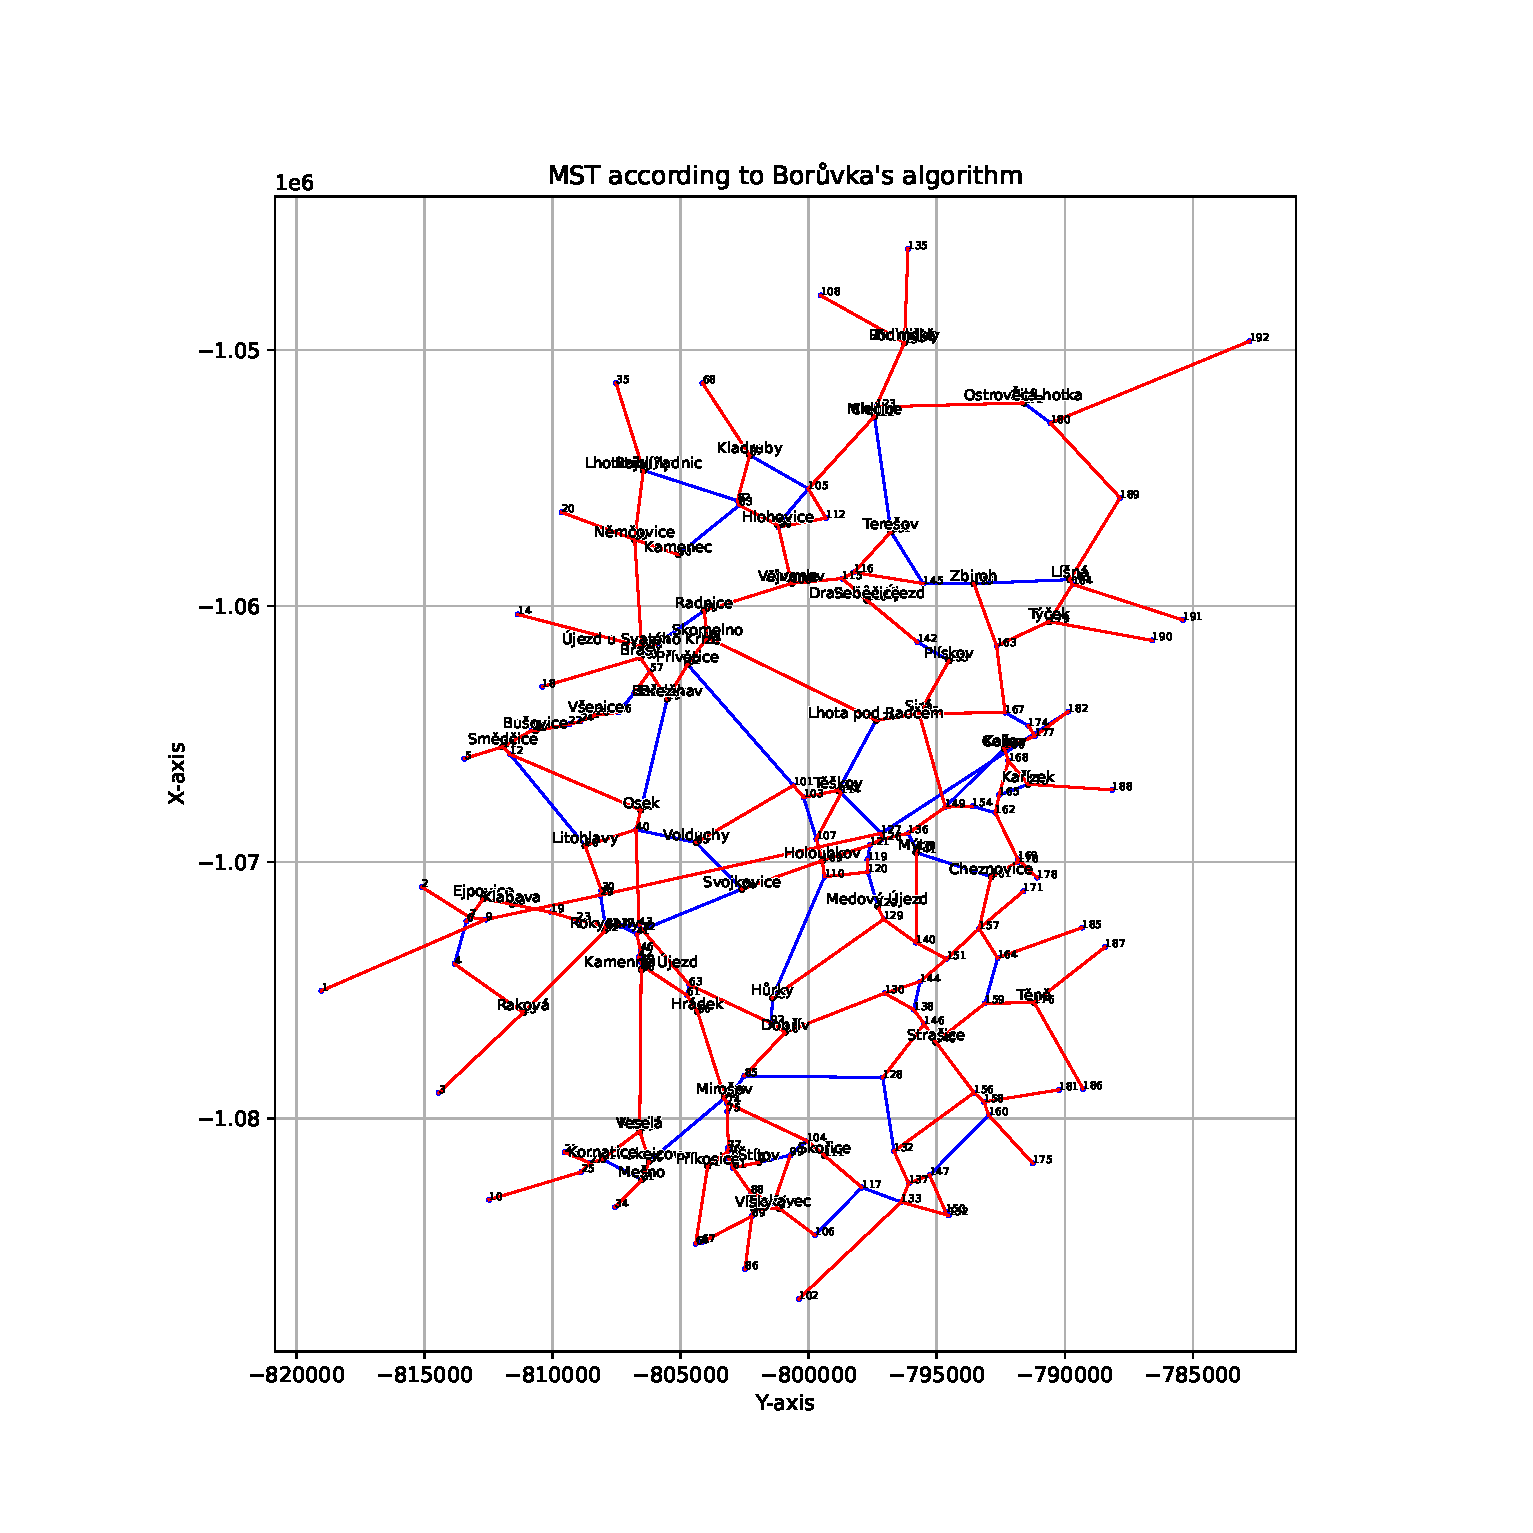
\includegraphics[width=0.65\textwidth]{images/Figure_3_curvature.eps}
    \caption{Minimální kostra v ohodnoceném grafu podle klikatosti podle Borůvkova algoritmu}
\end{figure}
%%%%%%%%%%%%%%%%%%%%%%%%%%%%%%%%%%%%%%%%%%%%%%%%%%%%%%%%%%%%%%%%%%%%%%%%%%%%%%%
\begin{figure}[H]
    \centering
    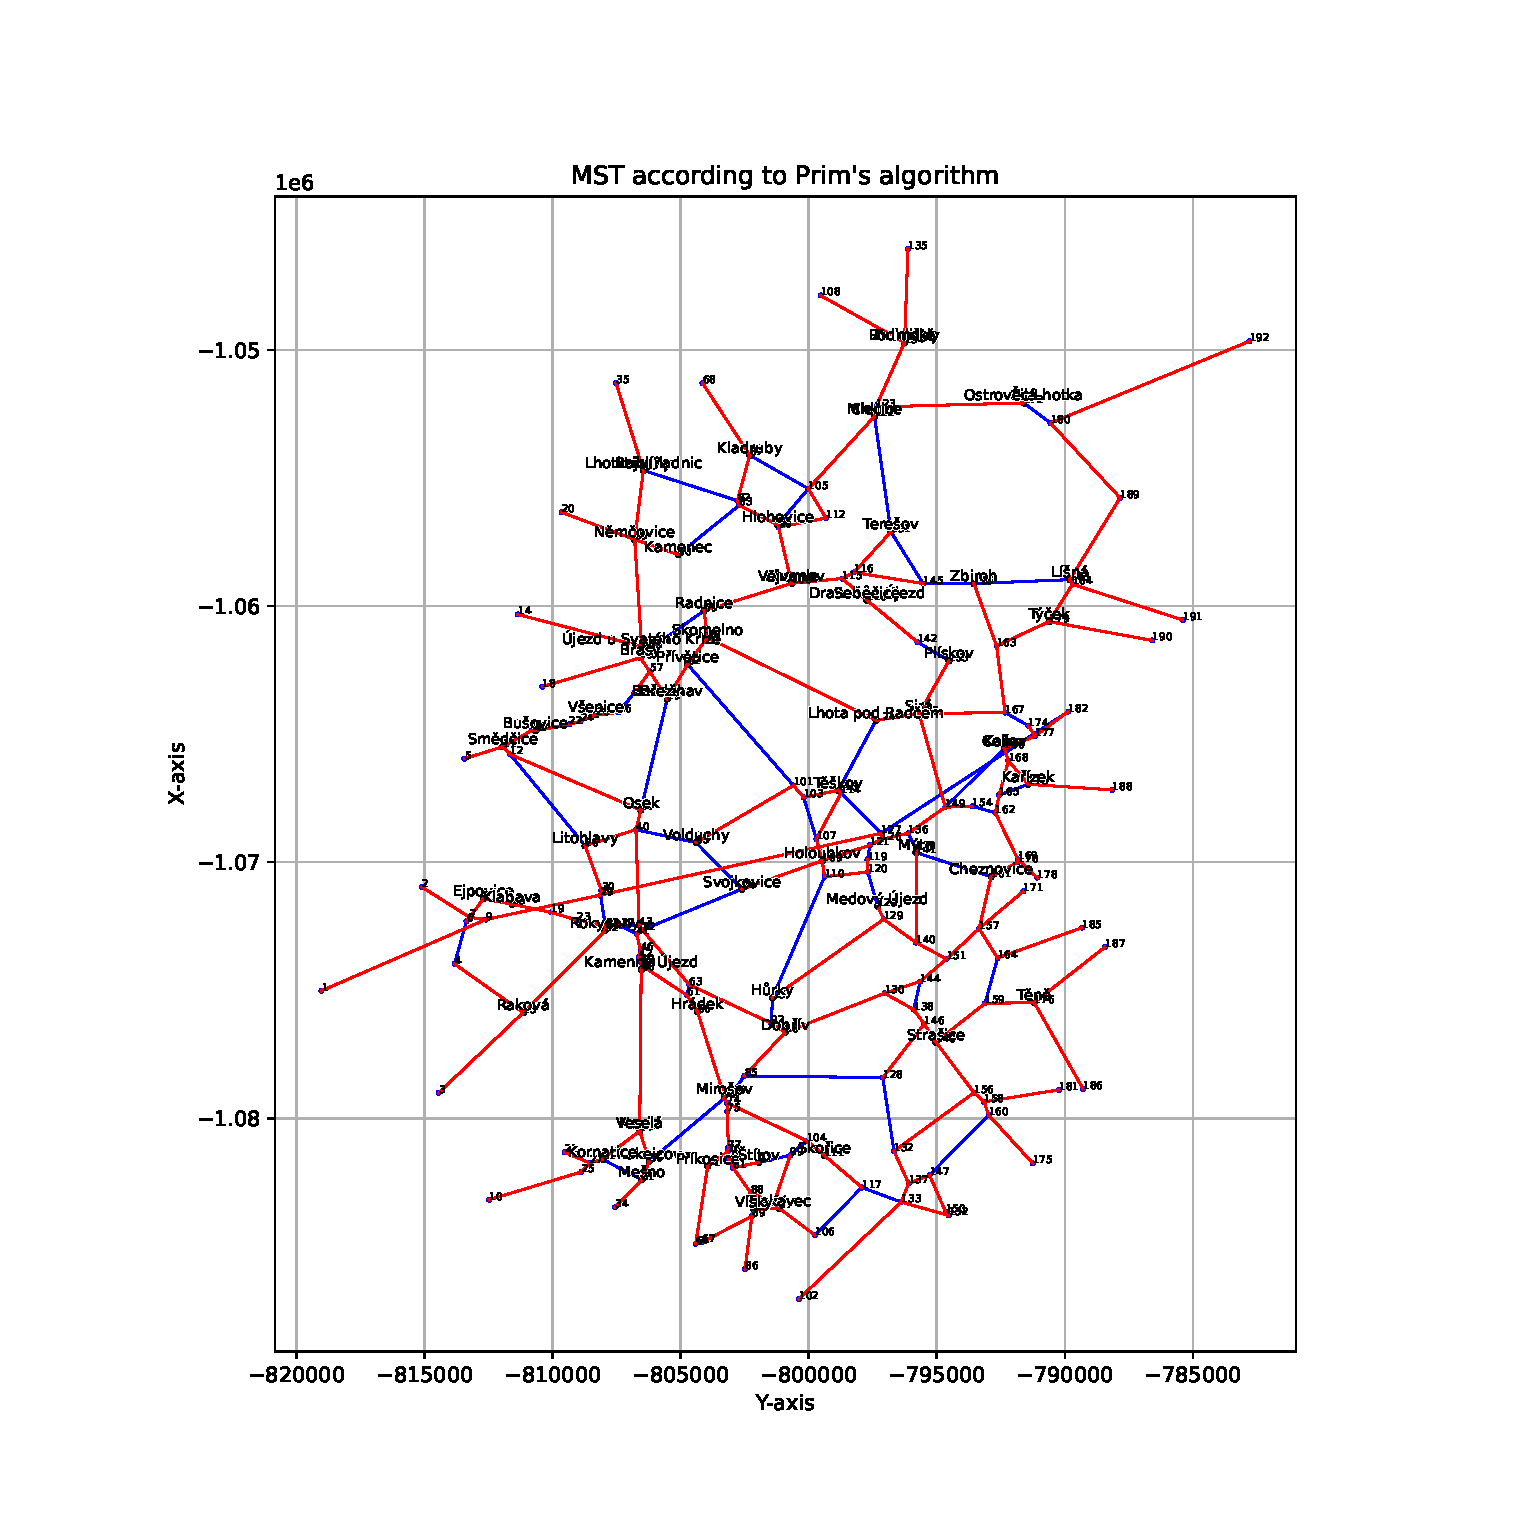
\includegraphics[width=0.65\textwidth]{images/Figure_2_curvature.eps}
    \caption{Minimální kostra v ohodnoceném grafu podle délky podle Primova algoritmu}
\end{figure}
\begin{figure}[H]
    \centering
    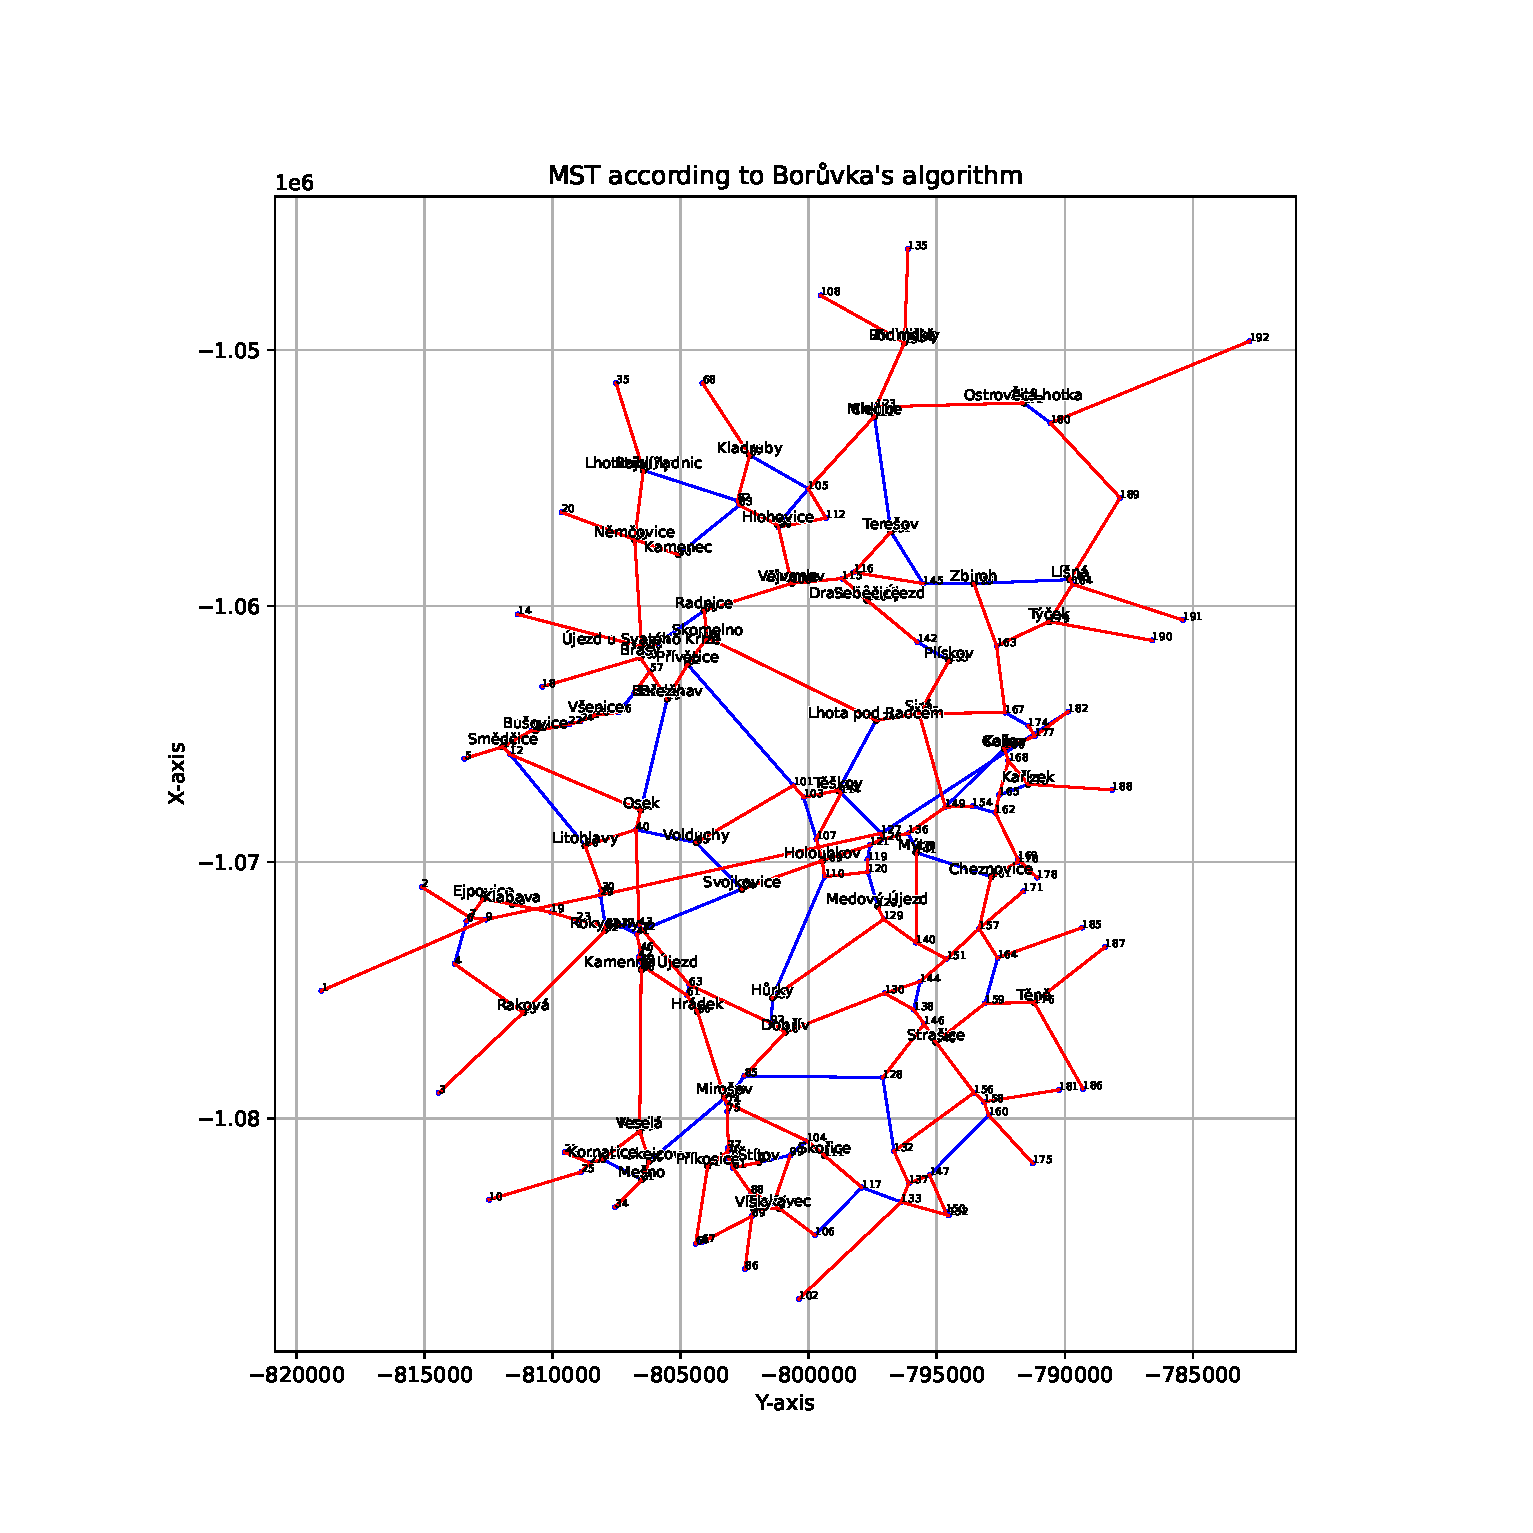
\includegraphics[width=0.65\textwidth]{images/Figure_3_curvature.eps}
    \caption{Minimální kostra v ohodnoceném grafu podle délky podle Borůvkova algoritmu}
\end{figure}
%%%%%%%%%%%%%%%%%%%%%%%%%%%%%%%%%%%%%%%%%%%%%%%%%%%%%%%%%%%%%%%%%%%%%%%%%%%%%%%
\begin{figure}[H]
    \centering
    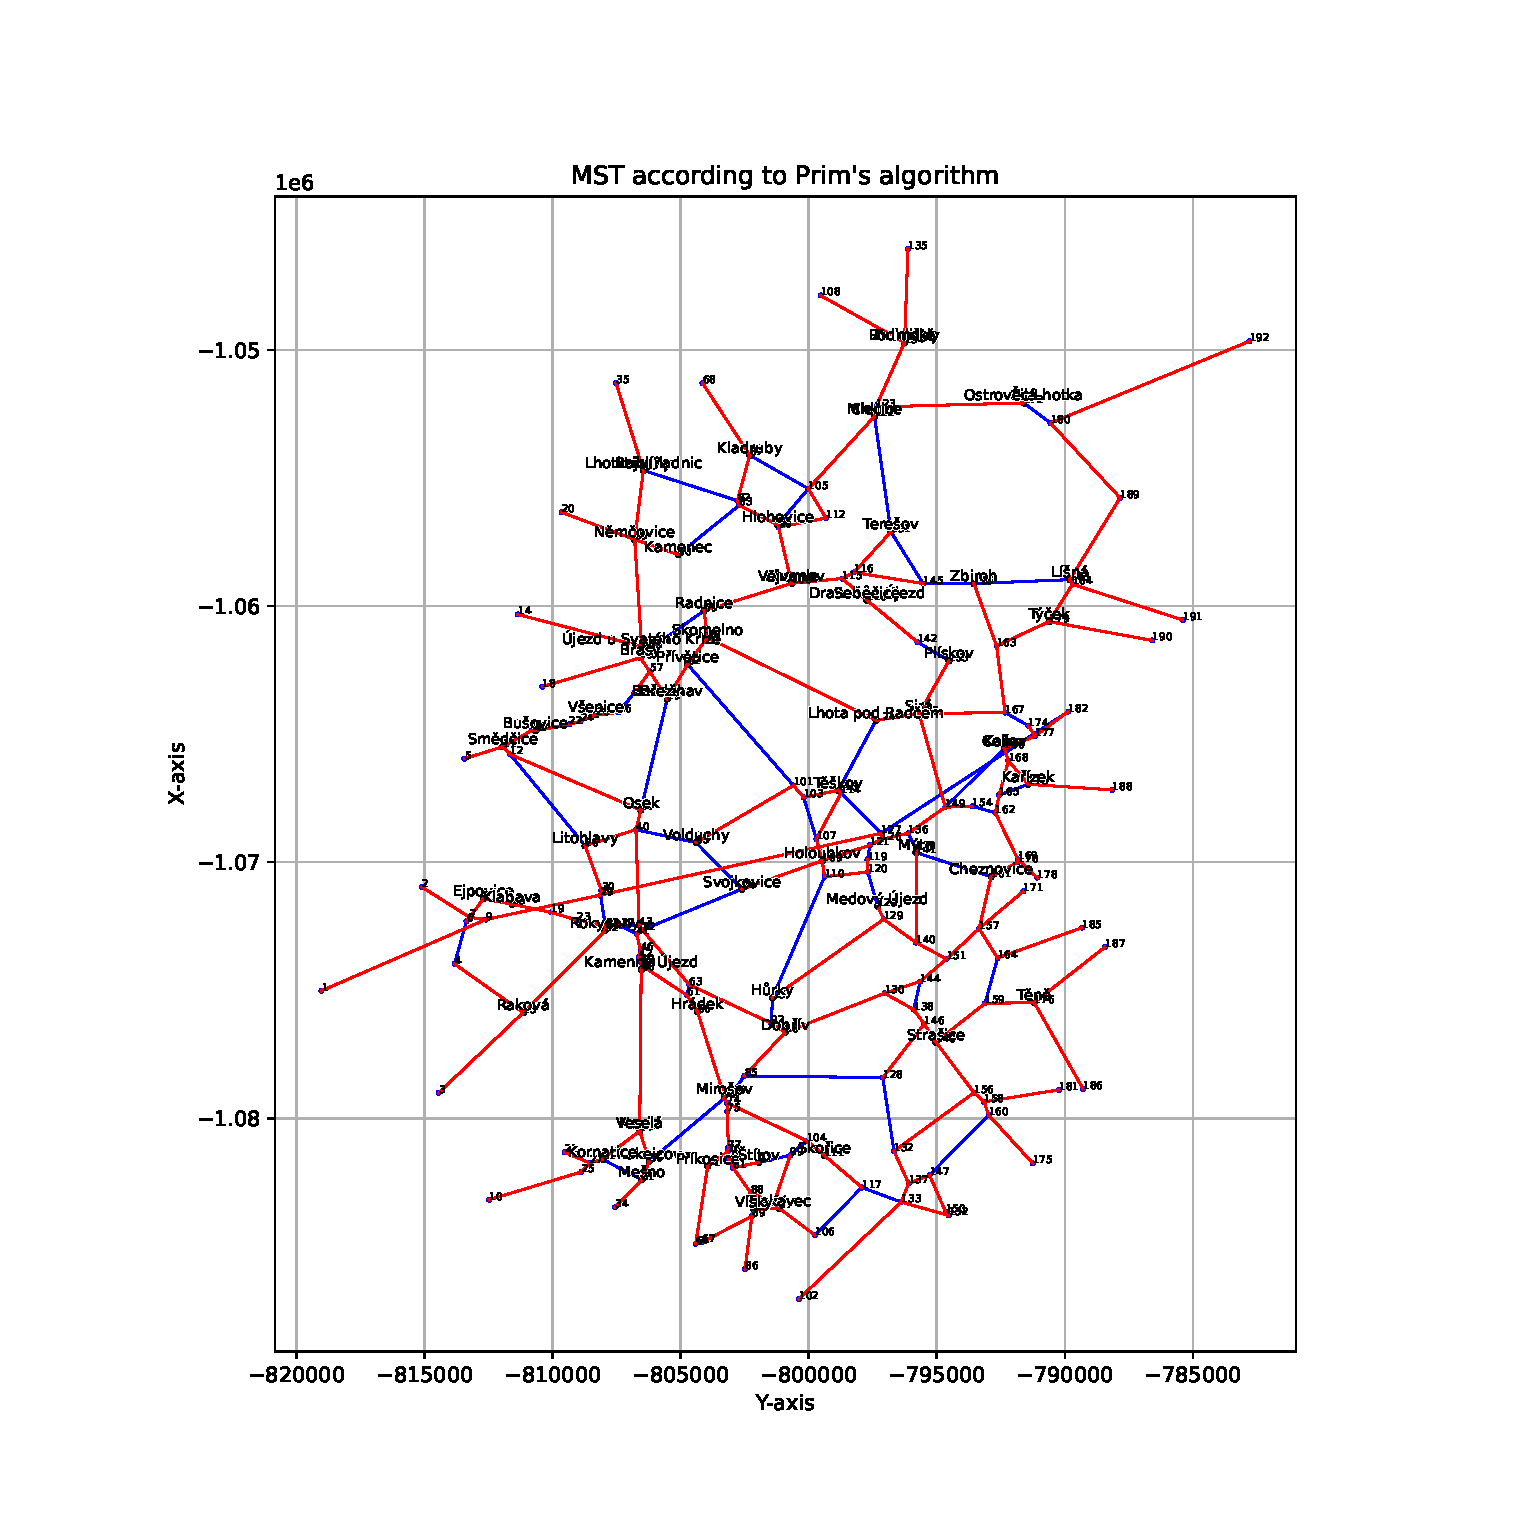
\includegraphics[width=0.65\textwidth]{images/Figure_2_curvature.eps}
    \caption{Minimální kostra v ohodnoceném grafu podle návrhové rychlosti podle Primova algoritmu}
\end{figure}
\begin{figure}[H]
    \centering
    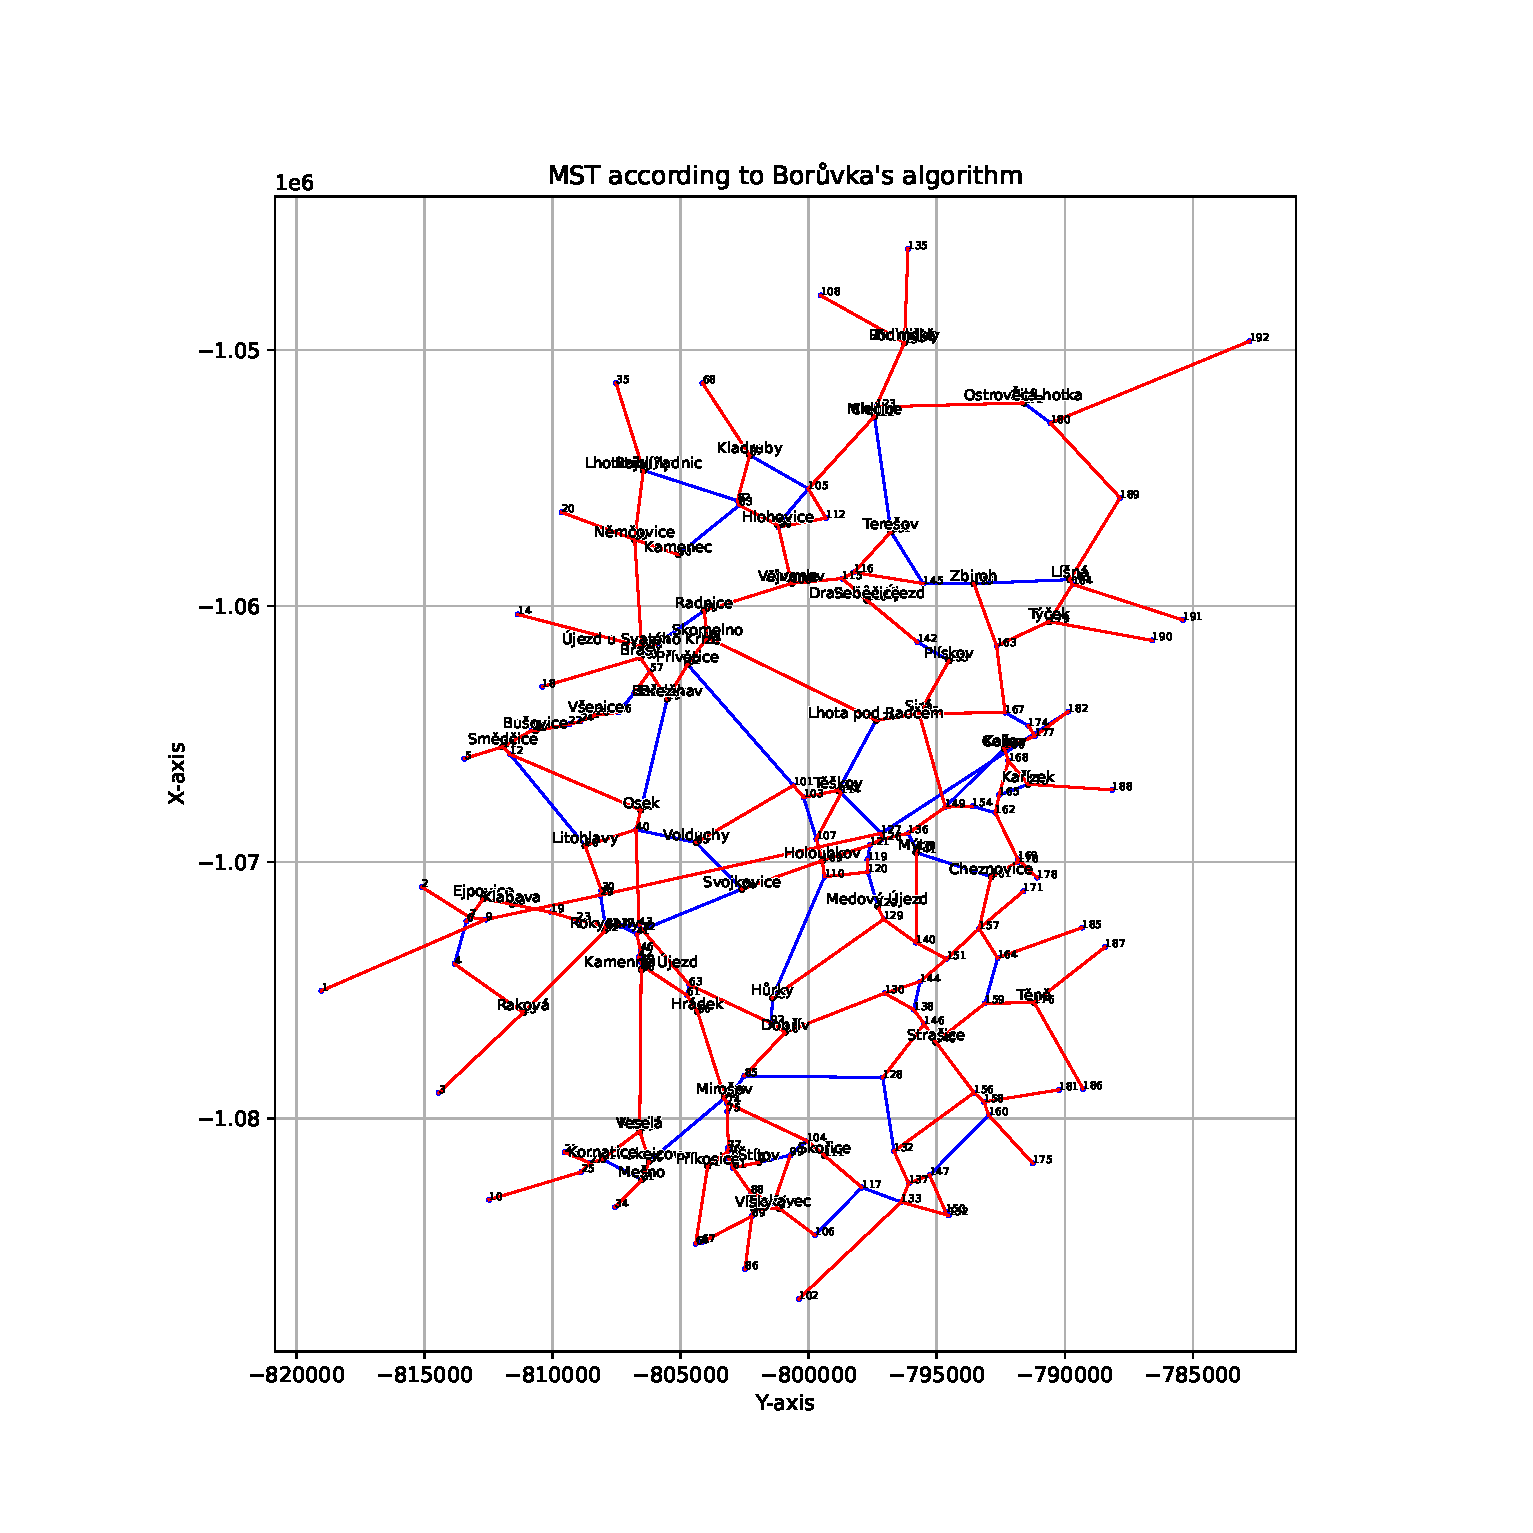
\includegraphics[width=0.65\textwidth]{images/Figure_3_curvature.eps}
    \caption{Minimální kostra v ohodnoceném grafu podle návrhové rychlosti podle Borůvkova algoritmu}
\end{figure}